\section{Filtro}
Una vez rectificada la señal el siguiente paso es suavizar y nivelar la
corriente directa pulsante. El método más sencillo para lograr esto es agregar
un condensador en paralelo a la carga. El condensador se cargará durante la fase
de conducción, almacenando así energia. Cuando el diodo se apaga, el condensador
comenzará a descargarse, transfiriendo asi su energia almacenada a la carga.

\subsection{Media onda}
El circuito con filtro de $470[\mu\text{F}]$ pueden verse en la
\textbf{figura~\ref{circuito05}} para el rectificador de media onda.

\begin{figure}[!h]
\centering
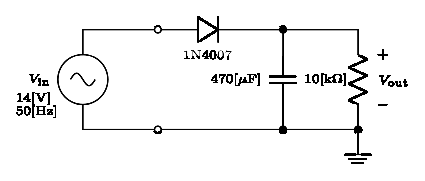
\includegraphics[scale=1]{diagramas/05.media_onda2.eps}
\caption{Rectificador de media onda con filtro.}
\label{circuito05}
\end{figure}

\subsubsection{Simulación}
Se utilizó el software \emph{Quite Universal Circuit Simulator.} versión 23.3.1
para la simulación del rectificador de media onda con filtro, este puede verse
en la \textbf{figura~\ref{simulacion05}}.

\begin{figure}[!h]
\centering
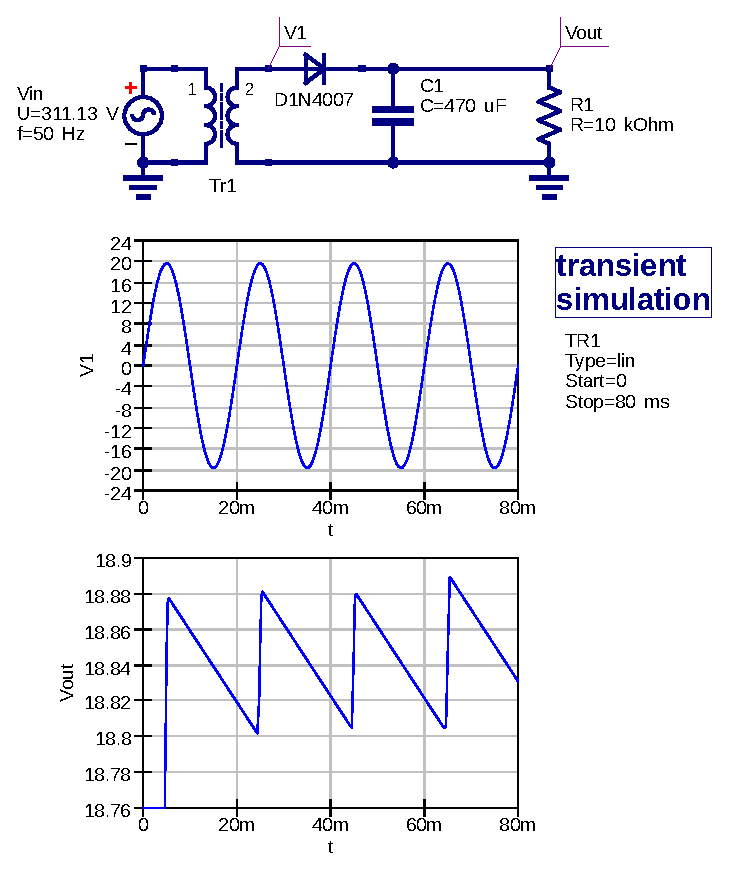
\includegraphics[scale=0.75]{simulacion/05.media_onda2.eps}
\caption{Simulación del rectificador de media onda con filtro.}
\label{simulacion05}
\end{figure}

\subsubsection{Laboratorio}
Se presenta el rectificador de media onda con filtro armado en laboratorio y su
medición de voltaje de salida en la carga, en la
\textbf{figura~\ref{laboratorio07}}.

\begin{figure}[!h]
\centering
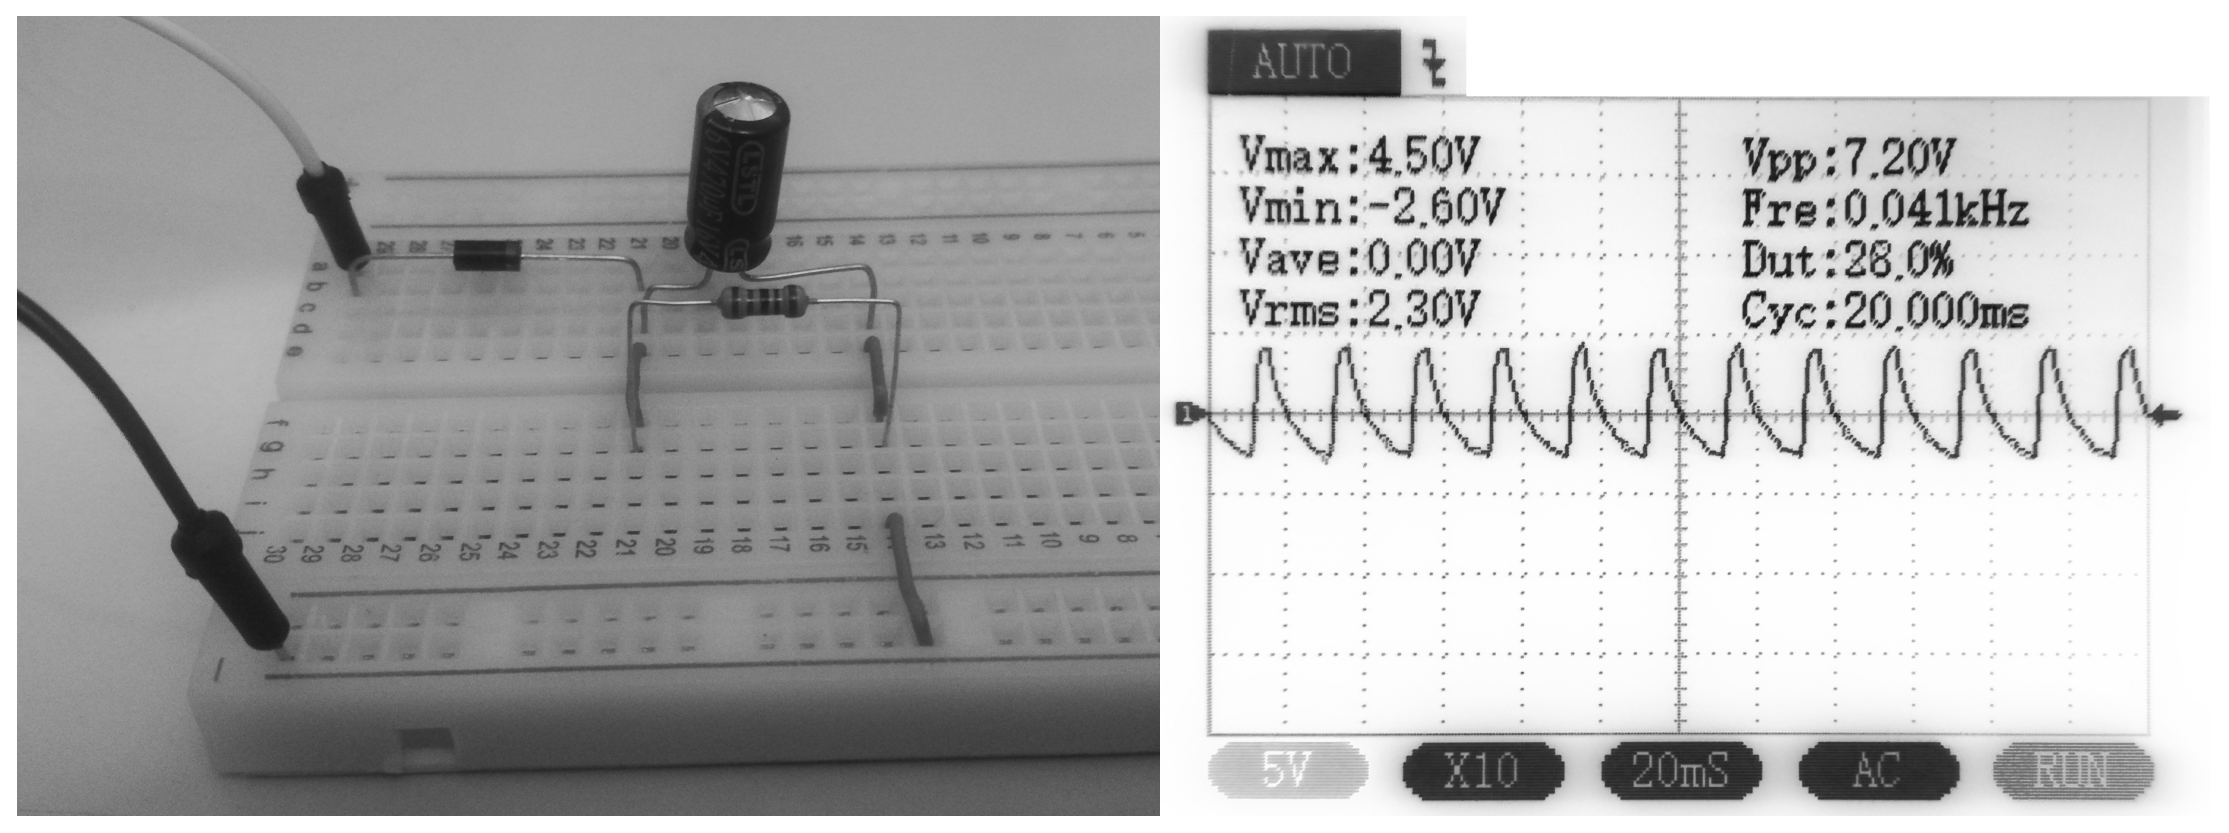
\includegraphics[scale=0.28]{fotos/05.media_onda2.eps}
\caption{Rectificador de media onda con filtro.}
\label{laboratorio07}
\end{figure}

\subsection{Onda completa con derivación central}
El circuito con filtro de $470[\mu\text{F}]$ pueden verse en la
\textbf{figura~\ref{circuito06}} para el rectificador de onda completa con
derivación central.

\begin{figure}[!h]
\centering
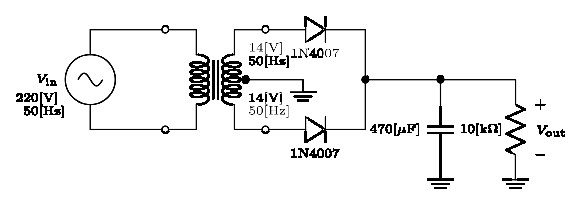
\includegraphics[scale=1]{diagramas/06.derivacion_central2.eps}
\caption{Rectificador de onda completa con transformador de \\
derivación central y filtro.}
\label{circuito06}
\end{figure}

\subsubsection{Simulación}
Se utilizó el software \emph{Quite Universal Circuit Simulator.} versión 23.3.1
para la simulación del rectificador de onda completa con transformador de
derivación central con filtro, este puede verse en la
\textbf{figura~\ref{simulacion06}}.

\begin{figure}[!h]
\centering
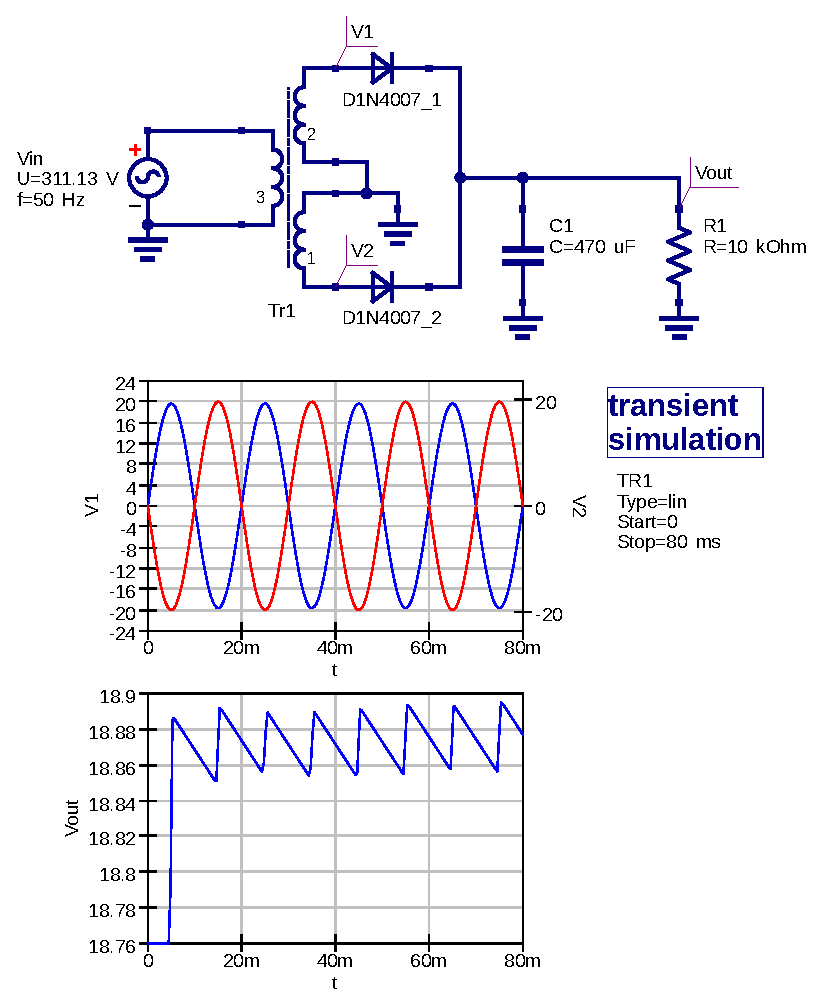
\includegraphics[scale=0.75]{simulacion/06.derivacion_central2.eps}
\caption{Simulación del rectificador de onda completa con \\
derivacion central y filtro.}
\label{simulacion06}
\end{figure}

\subsubsection{Laboratorio}
Se presenta el rectificador de onda completa con el transformador de derivación
central y filtro armado en laboratorio y su medición de voltaje de salida en la
carga, en la \textbf{figura~\ref{laboratorio08}}.

\begin{figure}[!h]
\centering
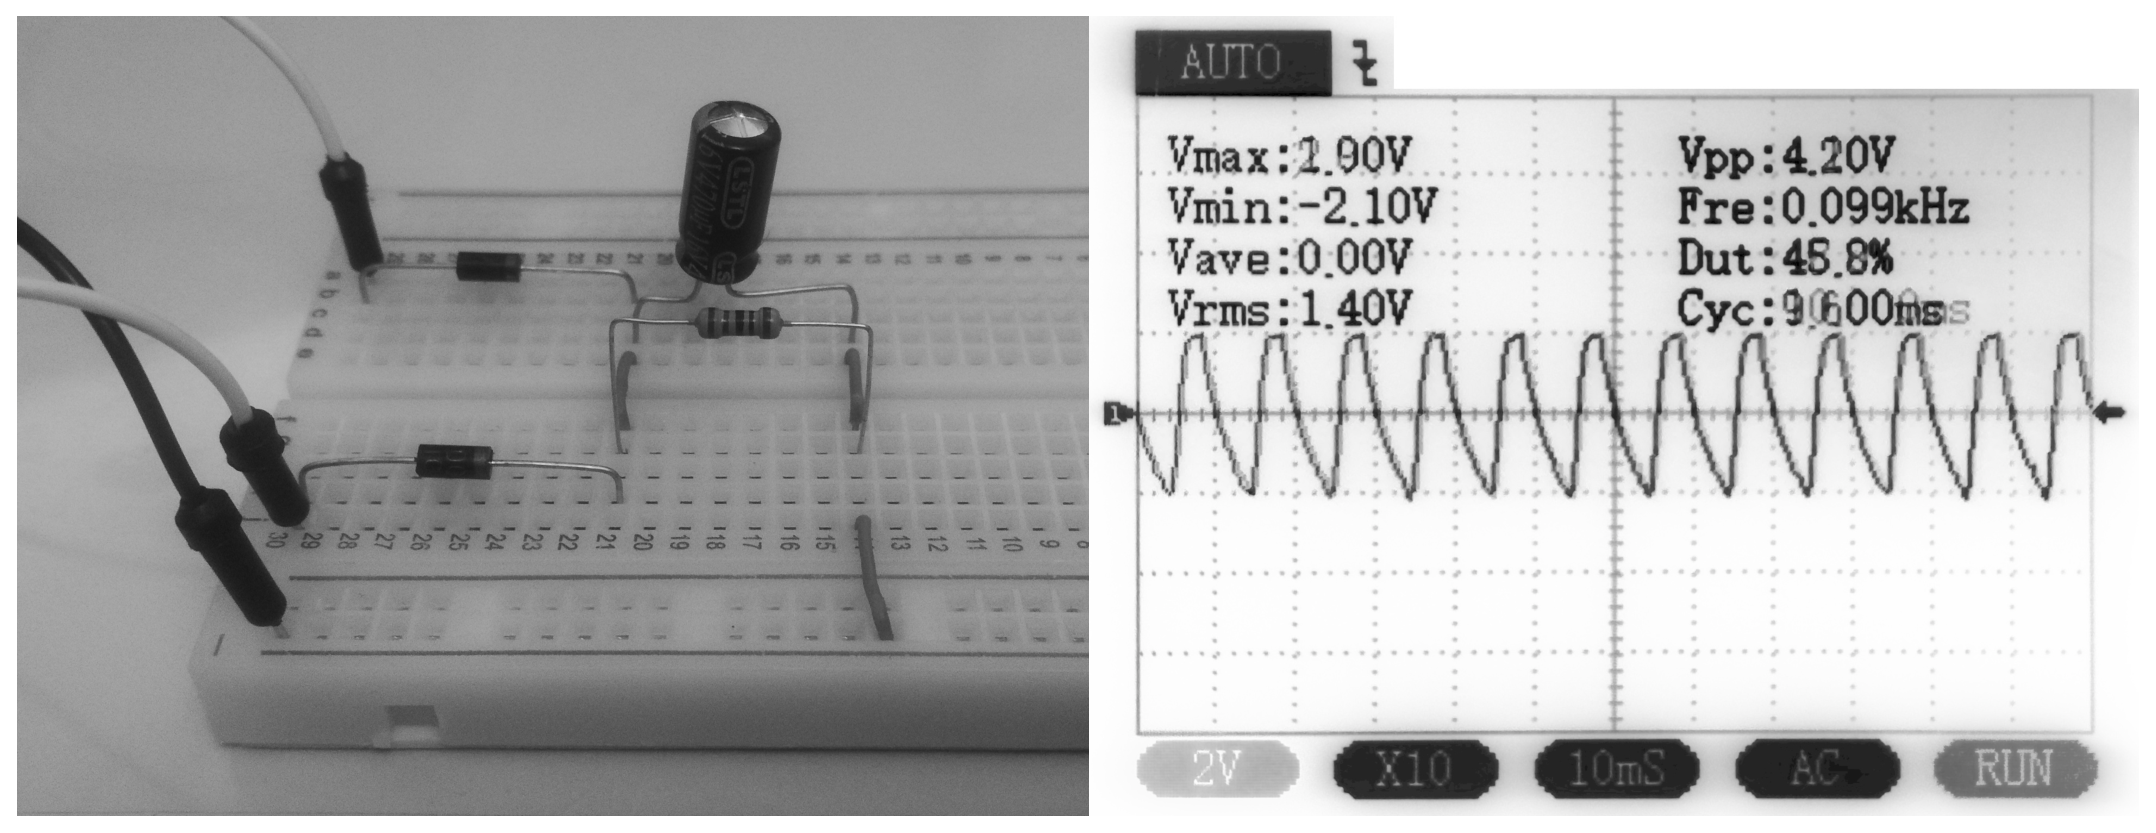
\includegraphics[scale=0.28]{fotos/06.derivacion_central2.eps}
\caption{Rectificador de onda completa con derivación central y filtro.}
\label{laboratorio08}
\end{figure}

\subsection{Onda completa de puente}
El circuito con filtro de $470[\mu\text{F}]$ pueden verse en la
\textbf{figura~\ref{circuito07}} para el rectificador de onda completa de
puente.

\begin{figure}[!h]
\centering
\includegraphics[scale=1]{diagramas/07.onda_completa2.eps}
\caption{Rectificador de onda completa con puente y filtro.}
\label{circuito07}
\end{figure}

\subsubsection{Simulación}
Se utilizó el software \emph{Quite Universal Circuit Simulator.} versión 23.3.1
para la simulación del rectificador de onda completa con filtro, este puede
verse en la \textbf{figura~\ref{simulacion07}}.

\begin{figure}[!h]
\centering
\includegraphics[scale=0.75]{simulacion/07.onda_completa2.eps}
\caption{Simulación del rectificador de onda completa con puente y filtro.}
\label{simulacion07}
\end{figure}

\subsubsection{Laboratorio}
Se presenta el rectificador de onda completa con puente y filtro armado en
laboratorio y su medición de voltaje de salida en la carga, en la
\textbf{figura~\ref{laboratorio09}}.

\begin{figure}[!h]
\centering
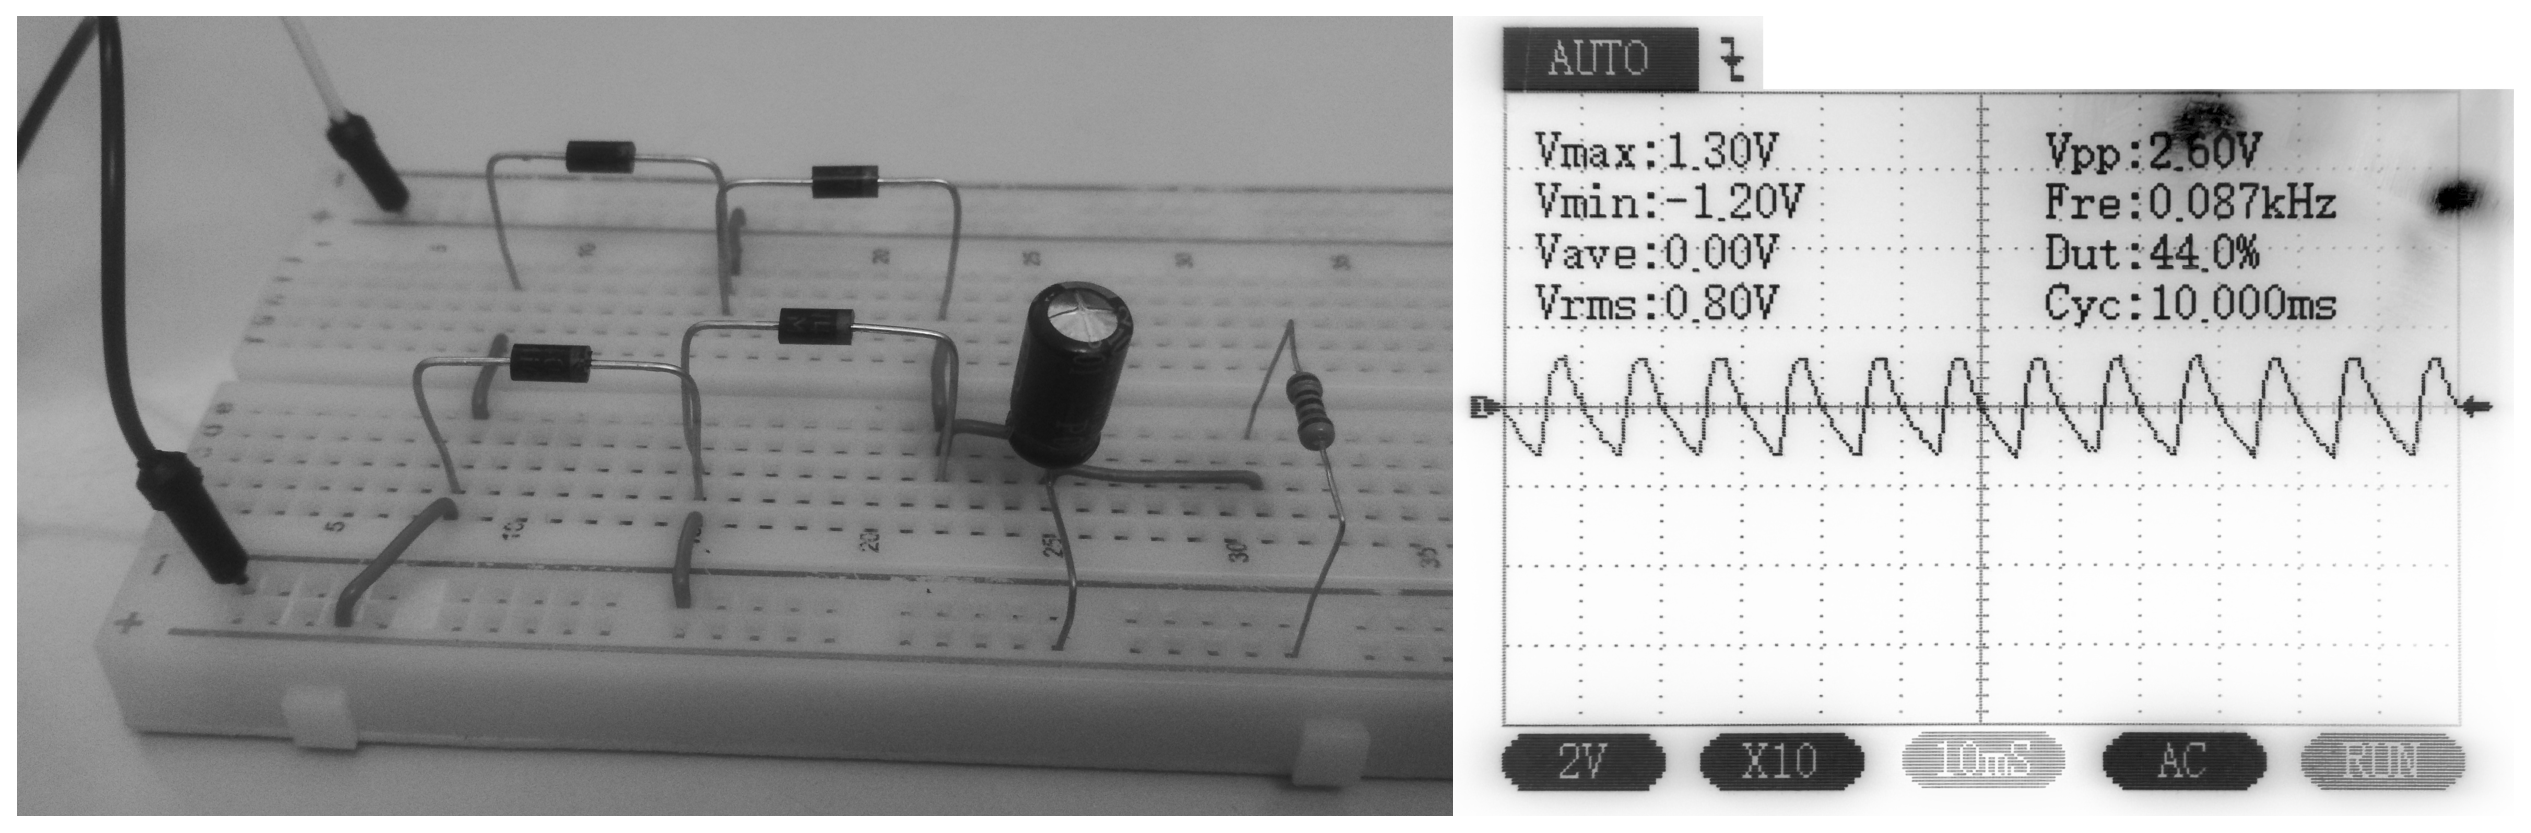
\includegraphics[scale=0.28]{fotos/07.onda_completa2.eps}
\caption{Rectificador de onda completa con puente y filtro.}
\label{laboratorio09}
\end{figure}

